\documentclass[aspectratio=169, 10pt]{beamer}

% --- Packages ---
\usepackage[utf8]{inputenc}
\usepackage{tikz}
\usepackage{pgfplots}
\usepackage{amsmath, amssymb, amsfonts}
\usepackage{booktabs}
\usepackage{bm}
\usepackage{xcolor}
\usetikzlibrary{arrows.meta, calc, positioning, shapes.geometric, decorations.pathreplacing, backgrounds, fit, shadows, patterns, shapes.arrows, angles, quotes, decorations.markings}
\pgfplotsset{compat=1.17}

% NYU Colors
\definecolor{nyupurple}{RGB}{87,46,140}
\definecolor{nyuheader}{RGB}{172,159,195}
\definecolor{nyufooter}{RGB}{189,178,211}

% Theme
\usetheme{default}
\setbeamertemplate{navigation symbols}{}

% Itemize
\setbeamercolor{itemize item}{fg=nyupurple}
\setbeamercolor{itemize subitem}{fg=nyupurple}
\setbeamercolor{itemize subsubitem}{fg=nyupurple}
\setbeamertemplate{itemize item}{\textbullet}
\setbeamertemplate{itemize subitem}{\textbullet}
\setbeamertemplate{itemize subsubitem}{\textbullet}

% Blocks
\setbeamercolor{block title}{fg=white, bg=nyupurple}
\setbeamercolor{block body}{fg=black, bg=nyuheader!30}
\setbeamercolor{block title alerted}{fg=white, bg=red!70}
\setbeamercolor{block body alerted}{fg=black, bg=red!10}
\setbeamercolor{block title example}{fg=white, bg=green!50!black}
\setbeamercolor{block body example}{fg=black, bg=green!10}

% Diagram colors
\definecolor{darkblue}{RGB}{0,51,102}
\definecolor{brightblue}{RGB}{0,102,204}
\definecolor{lightblue}{RGB}{153,204,255}
\definecolor{darkgreen}{RGB}{0,102,51}
\definecolor{accentred}{RGB}{192,0,0}
\definecolor{accentgreen}{RGB}{0,128,0}
\definecolor{accentorange}{RGB}{255,128,0}

% Commands
\newcommand{\vect}[1]{\boldsymbol{#1}}
\newcommand{\mat}[1]{\mathbf{#1}}

% Header
\makeatletter
\setbeamertemplate{frametitle}{%
    \nointerlineskip%
    \begin{beamercolorbox}[wd=\paperwidth,ht=0.7cm,dp=0.15cm,rightskip=0.5cm]{frametitle}
        \hspace{0.3cm}\usebeamerfont{frametitle}\insertframetitle%
        \hfill%
        \raisebox{0.08cm}{{\bfseries\sffamily\color{nyupurple}NYU}}%
    \end{beamercolorbox}%
}
\makeatother
\setbeamercolor{frametitle}{fg=black, bg=nyuheader}
\setbeamerfont{frametitle}{size=\large}

% Footer
\setbeamertemplate{footline}{%
    \begin{tikzpicture}[remember picture, overlay]
        \fill[nyufooter] ([yshift=0.6cm]current page.south west) rectangle ([xshift=5cm]current page.south east);
        \fill[nyufooter!70] ([yshift=0.6cm, xshift=5cm]current page.south west) rectangle ([xshift=10.5cm]current page.south east);
        \fill[nyufooter!40] ([yshift=0.6cm, xshift=10.5cm]current page.south west) rectangle (current page.south east);
        \node[anchor=west, font=\small] at ([xshift=0.3cm, yshift=0.3cm]current page.south west) {Dr.\ Aliasghar Arab};
        \node[anchor=center, font=\small] at ([yshift=0.3cm]current page.south) {Autonomous Mobile Robots};
        \node[anchor=east, font=\small] at ([xshift=-0.3cm, yshift=0.3cm]current page.south east) {LECTURE 6 -- FALL 2025 \quad \insertframenumber{} / \inserttotalframenumber};
    \end{tikzpicture}%
}

% Title page
\defbeamertemplate*{title page}{customized}[1][]
{
    \begin{tikzpicture}[remember picture, overlay]
        \node[anchor=north east] at ([xshift=-0.8cm, yshift=-0.8cm]current page.north east) {%
            {\bfseries\sffamily\Large\color{nyupurple}NYU}%
            {\sffamily\normalsize\color{black}\ \ TANDON SCHOOL OF ENGINEERING}%
        };
    \end{tikzpicture}
    
    \vspace{2cm}
    \centering
    {\Large\bfseries\inserttitle\par}
    \vspace{0.3cm}
    {\insertsubtitle\par}
    \vspace{1cm}
    {\insertauthor\par}
    \vspace{0.3cm}
    {\small\insertinstitute\par}
    \vspace{0.5cm}
    {\insertdate\par}
}

% Title info
\title{Autonomous Mobile Robots}
\subtitle{Lecture 6: Nonlinear Control Methods}
\author{Dr.\ Aliasghar Arab}
\institute{NYU Tandon School of Engineering}
\date{Fall 2025}

\begin{document}

% ==================== TITLE SLIDE ====================
{
\setbeamertemplate{footline}{}
\begin{frame}[plain]
\titlepage
\end{frame}
}

% ==================== OVERVIEW ====================
\begin{frame}{Lecture Overview}
\begin{block}{Today's Topics}
\begin{itemize}
    \item Feedback Linearization
    
    \vspace{0.3cm}
    \item Robust Control
    
    \vspace{0.3cm}
    \item Sliding Mode Control
    
    \vspace{0.3cm}
    \item Adaptive Control
\end{itemize}
\end{block}

\vspace{0.5cm}
\textbf{Goal:} Control nonlinear systems in the presence of uncertainties and unknown parameters.
\end{frame}

% ==================== PART 1: FEEDBACK LINEARIZATION ====================
\begin{frame}{Part 1: Feedback Linearization}
\begin{center}
\vspace{1cm}
{\Large\color{nyupurple}\textbf{Feedback Linearization}}

\vspace{0.5cm}
{\large Controllability of Nonlinear Systems via Lie Brackets}
\end{center}
\end{frame}

\begin{frame}{Controllability: Linear Systems}
\begin{block}{Linear System}
\[\dot{x} = Ax + bu\]
\end{block}

\vspace{0.3cm}
\begin{block}{Controllability Matrix}
\[\mathcal{C} = \begin{bmatrix} b & Ab & A^2b & \cdots & A^{n-1}b \end{bmatrix}\]
\end{block}

\vspace{0.3cm}
\begin{block}{Controllability Condition}
The system is \textbf{controllable} if and only if:
\[\text{rank}(\mathcal{C}) = n \quad \Leftrightarrow \quad |\mathcal{C}| \neq 0\]
\end{block}
\end{frame}

\begin{frame}{Controllability: Nonlinear Systems}
\begin{block}{Nonlinear Control-Affine System}
\[\dot{x} = f(x) + g(x)u\]
\end{block}

\vspace{0.3cm}
\begin{block}{Controllability via Lie Brackets}
\[\mathcal{C} = \{ad_f^0 g, \; ad_f^1 g, \; ad_f^2 g, \; \ldots, \; ad_f^{n-1} g\}\]
\end{block}

\vspace{0.3cm}
The \textbf{Lie bracket} is the nonlinear analog of the $A^k b$ terms in linear controllability.
\end{frame}

\begin{frame}{Lie Bracket Definition}
\begin{block}{Definition}
For vector fields $f(x)$ and $g(x)$, the \textbf{Lie bracket} is:
\[[f,g] = \frac{\partial g}{\partial x}f - \frac{\partial f}{\partial x}g\]
\end{block}

\vspace{0.5cm}
\begin{block}{Iterated Lie Brackets (ad notation)}
\begin{align*}
ad_f^0 g &= g \\[0.2cm]
ad_f^1 g &= [f,g] \\[0.2cm]
ad_f^2 g &= [f,[f,g]] \\[0.2cm]
&\vdots
\end{align*}
\end{block}
\end{frame}

\begin{frame}{Controllability Distribution}
\begin{block}{Distribution}
\[\Delta = \text{span}\{g, \; [f,g], \; [f,[f,g]], \; \ldots\}\]
\end{block}

\vspace{0.5cm}
\begin{block}{Controllability Rank Condition}
The system $\dot{x} = f(x) + g(x)u$ is \textbf{locally controllable} at $x_0$ if:
\[\dim(\Delta(x_0)) = n\]
\end{block}

\vspace{0.3cm}
This is analogous to the rank condition for linear systems.
\end{frame}

\begin{frame}{Feedback Linearization Concept}
\begin{center}
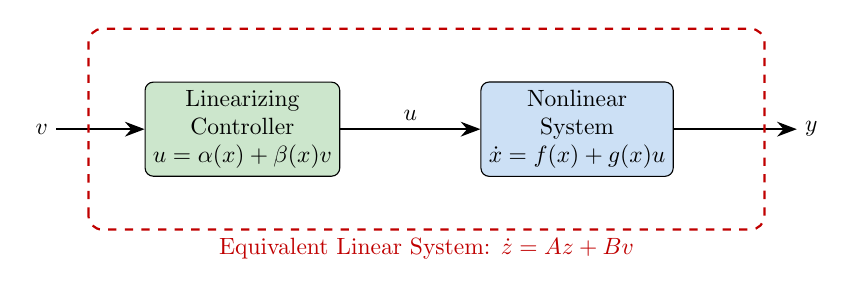
\begin{tikzpicture}[
    block/.style={draw, fill=nyuheader!30, rectangle, minimum height=1.2cm, minimum width=2.8cm, align=center, rounded corners=3pt},
    arrow/.style={-{Stealth[length=2.5mm]}, thick},
    scale=0.85, transform shape
]
% Input
\node (v) at (-5.5,0) {$v$};

% Linearizing Controller
\node[block, fill=accentgreen!20] (linctrl) at (-2.5,0) {Linearizing\\Controller\\$u = \alpha(x) + \beta(x)v$};

% Nonlinear Plant
\node[block, fill=brightblue!20] (plant) at (2.5,0) {Nonlinear\\System\\$\dot{x} = f(x) + g(x)u$};

% Output
\node (y) at (6,0) {$y$};

% Arrows
\draw[arrow] (v) -- (linctrl);
\draw[arrow] (linctrl) -- node[above] {$u$} (plant);
\draw[arrow] (plant) -- (y);

% Equivalent linear system box
\draw[dashed, thick, accentred, rounded corners=5pt] (-4.8,-1.5) rectangle (5.3,1.5);
\node[accentred, below] at (0.25,-1.5) {Equivalent Linear System: $\dot{z} = Az + Bv$};

\end{tikzpicture}
\end{center}

\vspace{0.3cm}
\begin{block}{Key Idea}
Find $u = \alpha(x) + \beta(x)v$ such that the closed-loop system is linear in new coordinates.
\end{block}
\end{frame}

\begin{frame}{Example: System Definition}
Consider the nonlinear system:
\[\dot{x} = f(x) + g(x)u\]

\vspace{0.3cm}
Where $x = \begin{bmatrix} x_1 \\ x_2 \end{bmatrix}$ and:

\vspace{0.3cm}
\[f(x) = \begin{bmatrix}
x_2 \\
x_1^2 + 2x_1x_2
\end{bmatrix}, \qquad 
g(x) = \begin{bmatrix}
x_1^2 \\
x_2^2
\end{bmatrix}\]
\end{frame}

\begin{frame}{Example: Jacobian of $g(x)$}
\begin{block}{Computing $\frac{\partial g}{\partial x}$}
\[\frac{\partial g}{\partial x} = 
\begin{bmatrix}
\dfrac{\partial g_1}{\partial x_1} & \dfrac{\partial g_1}{\partial x_2} \\[0.4cm]
\dfrac{\partial g_2}{\partial x_1} & \dfrac{\partial g_2}{\partial x_2}
\end{bmatrix} = 
\begin{bmatrix}
2x_1 & 0 \\[0.2cm]
0 & 2x_2
\end{bmatrix}\]
\end{block}
\end{frame}

\begin{frame}{Example: Jacobian of $f(x)$}
\begin{block}{Computing $\frac{\partial f}{\partial x}$}
\[\frac{\partial f}{\partial x} = 
\begin{bmatrix}
\dfrac{\partial f_1}{\partial x_1} & \dfrac{\partial f_1}{\partial x_2} \\[0.4cm]
\dfrac{\partial f_2}{\partial x_1} & \dfrac{\partial f_2}{\partial x_2}
\end{bmatrix} = 
\begin{bmatrix}
0 & 1 \\[0.2cm]
2x_1 + 2x_2 & 2x_1
\end{bmatrix}\]
\end{block}
\end{frame}

\begin{frame}{Example: Lie Bracket Calculation}
\[[f,g] = \frac{\partial g}{\partial x}f - \frac{\partial f}{\partial x}g\]

\vspace{0.3cm}
\begin{align*}
[f,g] &= \begin{bmatrix}
2x_1 & 0 \\
0 & 2x_2
\end{bmatrix}
\begin{bmatrix}
x_2 \\
x_1^2 + 2x_1x_2
\end{bmatrix} 
- \begin{bmatrix}
0 & 1 \\
2x_1 + 2x_2 & 2x_1
\end{bmatrix}
\begin{bmatrix}
x_1^2 \\
x_2^2
\end{bmatrix}
\end{align*}
\end{frame}

\begin{frame}{Example: Lie Bracket Calculation (cont.)}
First term:
\[\frac{\partial g}{\partial x}f = \begin{bmatrix}
2x_1 x_2 \\
2x_2(x_1^2 + 2x_1x_2)
\end{bmatrix}\]

\vspace{0.3cm}
Second term:
\[\frac{\partial f}{\partial x}g = \begin{bmatrix}
x_2^2 \\
(2x_1 + 2x_2)x_1^2 + 2x_1x_2^2
\end{bmatrix}\]

\vspace{0.3cm}
Therefore:
\[[f,g] = \begin{bmatrix}
2x_1 x_2 - x_2^2 \\
2x_1^2 x_2 + 4x_1 x_2^2 - 2x_1^3 - 2x_1^2 x_2 - 2x_1 x_2^2
\end{bmatrix}\]
\end{frame}

\begin{frame}{Example: Controllability Matrix}
\[\mathcal{C} = \begin{bmatrix}
g & [f,g]
\end{bmatrix} = 
\begin{bmatrix}
x_1^2 & 2x_1x_2 - x_2^2 \\[0.2cm]
x_2^2 & 2x_1^2x_2 - 2x_1^3
\end{bmatrix}\]

\vspace{0.5cm}
\begin{block}{Feedback Linearizability Conditions}
\begin{enumerate}
    \item $|\mathcal{C}| \neq 0$ (full rank)
    
    \vspace{0.2cm}
    \item The distribution $\{g, [f,g], \ldots, ad_f^{n-2}g\}$ must be \textbf{involutive}
\end{enumerate}
\end{block}
\end{frame}

% ==================== PART 2: ROBUST CONTROL ====================
\begin{frame}{Part 2: Robust Control}
\begin{center}
\vspace{1cm}
{\Large\color{nyupurple}\textbf{Robust Control}}

\vspace{0.5cm}
{\large Handling Bounded Uncertainties}
\end{center}
\end{frame}

\begin{frame}{Robust Control Problem}
\begin{block}{Real System with Uncertainties}
\[\dot{x} = f(x,u) + \Delta\]
where $\Delta$ represents unknown uncertainties.
\end{block}

\vspace{0.5cm}
\begin{exampleblock}{Example: Nonlinear Spring-Damper}
\[\ddot{x} + a\dot{x} + bx^3 + d(x) = u\]
\begin{itemize}
    \item $a\dot{x}$: damping term (uncertain coefficient)
    \item $bx^3$: nonlinear spring (uncertain coefficient)
    \item $d(x)$: unknown disturbance
\end{itemize}
\end{exampleblock}
\end{frame}

\begin{frame}{Robust Control Architecture}
\begin{center}
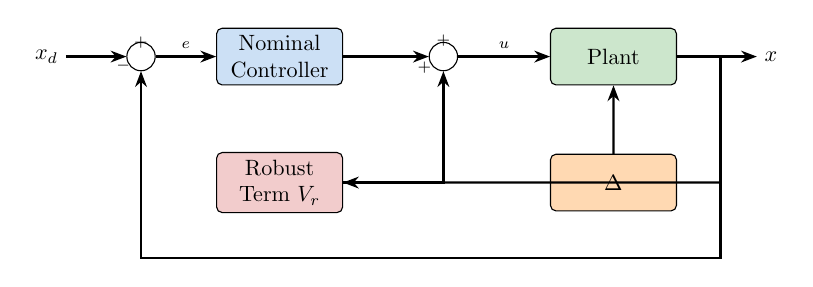
\begin{tikzpicture}[
    block/.style={draw, fill=nyuheader!30, rectangle, minimum height=0.9cm, minimum width=2cm, align=center, rounded corners=2pt},
    sumnode/.style={draw, circle, minimum size=0.45cm, fill=white},
    arrow/.style={-{Stealth[length=2mm]}, thick},
    scale=0.8, transform shape
]
% Reference
\node (xd) at (-5.5,0) {$x_d$};

% Sum node 1
\node[sumnode] (sum1) at (-4,0) {};
\node at (-4,0.22) {\scriptsize $+$};
\node at (-4.28,-0.15) {\scriptsize $-$};

% Nominal Controller
\node[block, fill=brightblue!20] (nomctrl) at (-1.8,0) {Nominal\\Controller};

% Robust Term
\node[block, fill=accentred!20] (robust) at (-1.8,-2) {Robust\\Term $V_r$};

% Sum node 2
\node[sumnode] (sum2) at (0.8,0) {};
\node at (0.8,0.25) {\scriptsize $+$};
\node at (0.5,-0.18) {\scriptsize $+$};

% Plant
\node[block, fill=accentgreen!20] (plant) at (3.5,0) {Plant};

% Uncertainty
\node[block, fill=accentorange!30] (uncert) at (3.5,-2) {$\Delta$};

% Output
\node (x) at (6,0) {$x$};

% Arrows
\draw[arrow] (xd) -- (sum1);
\draw[arrow] (sum1) -- node[above, font=\scriptsize] {$e$} (nomctrl);
\draw[arrow] (nomctrl) -- (sum2);
\draw[arrow] (robust) -| (sum2);
\draw[arrow] (sum2) -- node[above, font=\scriptsize] {$u$} (plant);
\draw[arrow] (plant) -- (x);
\draw[arrow] (uncert) -- (plant);

% Feedback
\draw[arrow] (5.2,0) -- (5.2,-3.2) -| (sum1);
\draw[arrow] (5.2,-2) -- (robust);

\end{tikzpicture}
\end{center}
\end{frame}

\begin{frame}{Control Objective}
\begin{block}{Goal}
Find control $u$ such that $x \to x_d$ despite uncertainties.
\end{block}

\vspace{0.4cm}
\begin{block}{Nominal Model}
\[\ddot{x} + \hat{a}\dot{x} + \hat{b}x^3 = u\]
where $\hat{a}$, $\hat{b}$ are estimated parameters.
\end{block}

\vspace{0.4cm}
\begin{block}{Proposed Controller}
\[u = \ddot{x}_d + \hat{a}\dot{x} + \hat{b}x^3 + k_d(\dot{x}_d - \dot{x}) + k_p(x_d - x) + V_r\]
\end{block}
\end{frame}

\begin{frame}{Error Dynamics Derivation}
Define tracking error: $e = x_d - x$

\vspace{0.3cm}
Substituting controller into the actual system dynamics:
\[\ddot{x}_d - \ddot{x} + k_d\dot{e} + k_p e = (a - \hat{a})\dot{x} + (b - \hat{b})x^3 + d(x) - V_r\]

\vspace{0.3cm}
\begin{block}{Error Dynamics}
\[\ddot{e} + k_d\dot{e} + k_p e = \Delta - V_r\]
where $\Delta = (a - \hat{a})\dot{x} + (b - \hat{b})x^3 + d(x)$
\end{block}
\end{frame}

\begin{frame}{State Space Representation}
Define state vector:
\[z = \begin{bmatrix} e \\ \dot{e} \end{bmatrix}\]

\vspace{0.3cm}
\begin{block}{State Space Form}
\[\dot{z} = Az + bw\]
\end{block}

\vspace{0.3cm}
Where:
\[A = \begin{bmatrix}
0 & 1 \\ -k_p & -k_d
\end{bmatrix}, \quad b = \begin{bmatrix} 0 \\ 1 \end{bmatrix}\]

\[w = (a - \hat{a})\dot{x} + (b - \hat{b})x^3 + d(x) - V_r\]
\end{frame}

\begin{frame}{Lyapunov Stability Analysis}
\begin{block}{Lyapunov Function Candidate}
\[V = \frac{1}{2} z^T P z\]
where $P > 0$ satisfies $A^T P + PA = -Q$ for some $Q > 0$.
\end{block}

\vspace{0.4cm}
\begin{block}{Time Derivative}
\begin{align*}
\dot{V} &= \frac{1}{2}[\dot{z}^T P z + z^T P \dot{z}] \\[0.2cm]
&= \frac{1}{2} z^T[A^T P + P A] z + z^T P b w \\[0.2cm]
&= -\frac{1}{2} z^T Q z + z^T P b w
\end{align*}
\end{block}
\end{frame}

\begin{frame}{Uncertainty Bounds}
\begin{block}{Assumptions on Uncertainty}
\begin{itemize}
    \item $|a - \hat{a}| < \alpha$
    
    \vspace{0.2cm}
    \item $|b - \hat{b}| < \beta$
    
    \vspace{0.2cm}
    \item $|d(x)| < \rho$
\end{itemize}
\end{block}

\vspace{0.4cm}
\begin{block}{Total Uncertainty Bound}
\[|(a - \hat{a})\dot{x} + (b - \hat{b})x^3 + d(x)| < \alpha|\dot{x}| + \beta|x|^3 + \rho = F(x, \dot{x})\]
\end{block}
\end{frame}

\begin{frame}{Robust Control Law}
\begin{block}{Robust Term Design}
\[V_r = \frac{z^T P b}{|z^T P b|} F(x, \dot{x})\]
\end{block}

\vspace{0.3cm}
This choice ensures:
\[z^T P b \cdot w < 0\]

\vspace{0.3cm}
\begin{block}{Stability Guarantee}
With this $V_r$:
\[\dot{V} = -\frac{1}{2} z^T Q z + z^T P b w < 0\]
guaranteeing asymptotic stability.
\end{block}
\end{frame}

% ==================== PART 3: SLIDING MODE CONTROL ====================
\begin{frame}{Part 3: Sliding Mode Control}
\begin{center}
\vspace{1cm}
{\Large\color{nyupurple}\textbf{Sliding Mode Control}}

\vspace{0.5cm}
{\large Robustness Through Discontinuous Control}
\end{center}
\end{frame}

\begin{frame}{Sliding Surface Definition}
\begin{block}{Sliding Surface}
\[S = \dot{e} + \lambda e\]
where $\lambda > 0$ is a design parameter.
\end{block}

\vspace{0.4cm}
\begin{block}{Control Objective}
Design control such that $S \to 0$.
\end{block}

\vspace{0.4cm}
\begin{block}{Convergence Property}
If $S = 0$: \quad $\dot{e} + \lambda e = 0 \implies e(t) = e(0)e^{-\lambda t} \to 0$
\end{block}
\end{frame}

\begin{frame}{Sliding Mode Phase Portrait}
\begin{center}
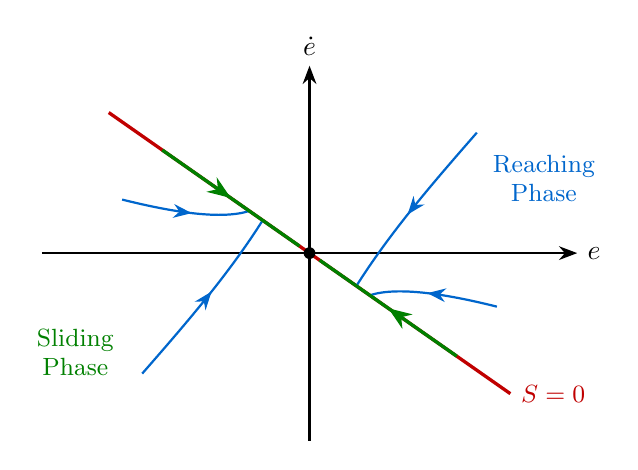
\begin{tikzpicture}[scale=0.85]
% Axes
\draw[thick, -{Stealth}] (-4,0) -- (4,0) node[right] {$e$};
\draw[thick, -{Stealth}] (0,-2.8) -- (0,2.8) node[above] {$\dot{e}$};

% Sliding surface S = 0: dot_e = -lambda * e
\draw[very thick, accentred] (-3,2.1) -- (3,-2.1) node[right, font=\small] {$S = 0$};

% Reaching phase trajectories
\draw[thick, brightblue, decoration={markings, mark=at position 0.55 with {\arrow{Stealth}}}, postaction={decorate}] 
    (2.5,1.8) .. controls (1.8,1) and (1.2,0.3) .. (0.7,-0.49);
\draw[thick, brightblue, decoration={markings, mark=at position 0.55 with {\arrow{Stealth}}}, postaction={decorate}] 
    (-2.5,-1.8) .. controls (-1.8,-1) and (-1.2,-0.3) .. (-0.7,0.49);
\draw[thick, brightblue, decoration={markings, mark=at position 0.55 with {\arrow{Stealth}}}, postaction={decorate}] 
    (2.8,-0.8) .. controls (2,-0.6) and (1.3,-0.5) .. (0.9,-0.63);
\draw[thick, brightblue, decoration={markings, mark=at position 0.55 with {\arrow{Stealth}}}, postaction={decorate}] 
    (-2.8,0.8) .. controls (-2,0.6) and (-1.3,0.5) .. (-0.9,0.63);

% Sliding phase along surface
\draw[very thick, accentgreen, decoration={markings, mark=at position 0.5 with {\arrow{Stealth}}}, postaction={decorate}] 
    (2.2,-1.54) -- (0.15,-0.105);
\draw[very thick, accentgreen, decoration={markings, mark=at position 0.5 with {\arrow{Stealth}}}, postaction={decorate}] 
    (-2.2,1.54) -- (-0.15,0.105);

% Labels
\node[brightblue, font=\small] at (3.5,1.3) {Reaching};
\node[brightblue, font=\small] at (3.5,0.9) {Phase};
\node[accentgreen, font=\small] at (-3.5,-1.3) {Sliding};
\node[accentgreen, font=\small] at (-3.5,-1.7) {Phase};

% Origin
\fill (0,0) circle (2.5pt);

\end{tikzpicture}
\end{center}
\end{frame}

\begin{frame}{Sliding Mode Stability}
\begin{block}{Lyapunov Function}
\[V = \frac{1}{2}S^2\]
\end{block}

\vspace{0.4cm}
\begin{block}{Reaching Condition}
We want:
\[\dot{V} = S\dot{S} = -\eta |S|, \quad \eta > 0\]
\end{block}

\vspace{0.4cm}
This implies:
\[\dot{S} = -\eta \, \text{sgn}(S)\]
\end{frame}

\begin{frame}{Sliding Mode Control: System Setup}
Consider the second-order system:
\[\ddot{x} = f(x) + u\]

\vspace{0.4cm}
Sliding surface derivative:
\[\dot{S} = \ddot{e} + \lambda \dot{e} = \ddot{x}_d - \ddot{x} + \lambda \dot{e}\]

\vspace{0.4cm}
Substituting dynamics:
\[\dot{S} = \ddot{x}_d - f(x) - u + \lambda \dot{e}\]
\end{frame}

\begin{frame}{Sliding Mode Control Law}
From the reaching condition $\dot{S} = -\eta \, \text{sgn}(S)$:
\[\ddot{x}_d - f(x) - u + \lambda \dot{e} = -\eta \, \text{sgn}(S)\]

\vspace{0.4cm}
\begin{block}{Control Law}
\[u = \ddot{x}_d - f(x) + \lambda \dot{e} + \eta \, \text{sgn}(S)\]
\end{block}

\vspace{0.3cm}
The $\text{sgn}(S)$ term creates the discontinuous switching action.
\end{frame}

\begin{frame}{Robust Sliding Mode Control}
For system with uncertainty:
\[\ddot{x} = \hat{f}(x) + \Delta + u, \quad |\Delta| < F\]

\vspace{0.4cm}
\begin{block}{Robust Control Law}
\[u = \ddot{x}_d - \hat{f}(x) + \lambda \dot{e} + (\eta + F) \, \text{sgn}(S)\]
\end{block}

\vspace{0.4cm}
This guarantees:
\[S\dot{S} < -\eta |S|\]
ensuring finite-time reaching of the sliding surface.
\end{frame}

% ==================== PART 4: ADAPTIVE CONTROL ====================
\begin{frame}{Part 4: Adaptive Control}
\begin{center}
\vspace{1cm}
{\Large\color{nyupurple}\textbf{Adaptive Control}}

\vspace{0.5cm}
{\large Online Parameter Estimation}
\end{center}
\end{frame}

\begin{frame}{Adaptive Control Problem}
\begin{exampleblock}{Example: Pendulum System}
\[I\ddot{\theta} + b\dot{\theta} + C\sin\theta = \tau\]
\begin{itemize}
    \item $I$: unknown inertia
    
    \vspace{0.2cm}
    \item $b$: unknown damping
    
    \vspace{0.2cm}
    \item $C$: unknown gravitational term
\end{itemize}
\end{exampleblock}

\vspace{0.4cm}
\begin{block}{Control Objective}
Design $\tau$ and parameter update laws to track desired trajectory $\theta_d$.
\end{block}
\end{frame}

\begin{frame}{Adaptive Control Architecture}
\begin{center}
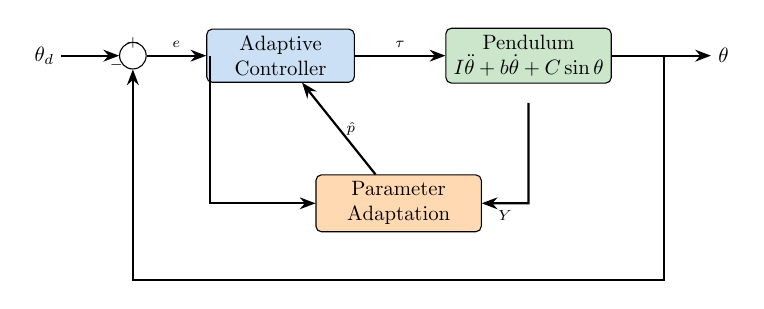
\begin{tikzpicture}[
    block/.style={draw, fill=nyuheader!30, rectangle, minimum height=0.9cm, minimum width=2.2cm, align=center, rounded corners=2pt},
    sumnode/.style={draw, circle, minimum size=0.45cm, fill=white},
    arrow/.style={-{Stealth[length=2mm]}, thick},
    scale=0.75, transform shape
]
% Reference
\node (thetad) at (-6,0) {$\theta_d$};

% Sum node
\node[sumnode] (sum1) at (-4.5,0) {};
\node at (-4.5,0.22) {\scriptsize $+$};
\node at (-4.78,-0.15) {\scriptsize $-$};

% Controller
\node[block, fill=brightblue!20, minimum width=2.5cm] (ctrl) at (-2,0) {Adaptive\\Controller};

% Plant
\node[block, fill=accentgreen!20, minimum width=2.8cm] (plant) at (2.2,0) {Pendulum\\$I\ddot{\theta} + b\dot{\theta} + C\sin\theta$};

% Output
\node (theta) at (5.5,0) {$\theta$};

% Parameter Estimator
\node[block, fill=accentorange!30, minimum width=2.8cm] (adapt) at (0,-2.5) {Parameter\\Adaptation};

% Arrows
\draw[arrow] (thetad) -- (sum1);
\draw[arrow] (sum1) -- node[above, font=\scriptsize] {$e$} (ctrl);
\draw[arrow] (ctrl) -- node[above, font=\scriptsize] {$\tau$} (plant);
\draw[arrow] (plant) -- (theta);

% Feedback to sum
\draw[arrow] (4.5,0) -- (4.5,-3.8) -| (sum1);

% Connection to adaptation
\draw[arrow] (-3.2,0) |- (adapt);
\draw[arrow] (adapt) -- node[right, font=\scriptsize] {$\hat{p}$} (ctrl);

% Regressor from plant
\draw[arrow] (2.2,-0.8) -- (2.2,-2.5) -- node[below, font=\scriptsize] {$Y$} (adapt);

\end{tikzpicture}
\end{center}
\end{frame}

\begin{frame}{Adaptive Control Law}
\begin{block}{Proposed Controller}
\[\tau = \hat{I}[\ddot{\theta}_d + k_d(\dot{\theta}_d - \dot{\theta}) + k_p(\theta_d - \theta)] + \hat{b}\dot{\theta} + \hat{C}\sin\theta\]
\end{block}

\vspace{0.5cm}
Where:
\begin{itemize}
    \item $\hat{I}, \hat{b}, \hat{C}$: parameter estimates (updated online)
    
    \vspace{0.2cm}
    \item $k_d, k_p$: feedback gains (fixed)
\end{itemize}
\end{frame}

\begin{frame}{Regressor Form}
Define parameter vector and regressor:
\[p = \begin{bmatrix} I \\ b \\ C \end{bmatrix}, \qquad Y = \begin{bmatrix} \ddot{\theta} \\ \dot{\theta} \\ \sin\theta \end{bmatrix}\]

\vspace{0.4cm}
Then the dynamics can be written as:
\[p^T Y = I\ddot{\theta} + b\dot{\theta} + C\sin\theta = \tau\]

\vspace{0.3cm}
This \textbf{linear-in-parameters} structure is key for adaptive control.
\end{frame}

\begin{frame}{Error System Representation}
Define error states: $x_1 = e = \theta_d - \theta$, $x_2 = \dot{e}$

\vspace{0.3cm}
\begin{block}{Error Dynamics}
\[\dot{x}_1 = x_2\]
\[\dot{x}_2 = -k_p x_1 - k_d x_2 + I^{-1}(p - \hat{p})^T Y\]
\end{block}

\vspace{0.3cm}
In matrix form:
\[\dot{x} = Ax + bw\]
where:
\[A = \begin{bmatrix} 0 & 1 \\ -k_p & -k_d \end{bmatrix}, \quad b = \begin{bmatrix} 0 \\ 1 \end{bmatrix}, \quad w = I^{-1}(p - \hat{p})^T Y\]
\end{frame}

\begin{frame}{Composite Lyapunov Function}
\begin{block}{Lyapunov Candidate}
\[V(x, \tilde{p}) = \frac{1}{2} x^T Q x + \frac{1}{2\gamma} \tilde{p}^T \tilde{p}\]
\end{block}

\vspace{0.3cm}
Where:
\begin{itemize}
    \item $\tilde{p} = p - \hat{p}$: parameter error
    
    \vspace{0.2cm}
    \item $Q > 0$: symmetric positive definite matrix
    
    \vspace{0.2cm}
    \item $\gamma > 0$: adaptation gain
\end{itemize}

\vspace{0.3cm}
\textit{Note: $Q$ is the Lyapunov matrix (distinct from sliding surface $S$).}
\end{frame}

\begin{frame}{Lyapunov Analysis}
Taking the time derivative:
\begin{align*}
\dot{V} &= x^T Q \dot{x} - \frac{1}{\gamma} \tilde{p}^T \dot{\hat{p}} \\[0.3cm]
&= x^T Q (Ax + bw) - \frac{1}{\gamma} \tilde{p}^T \dot{\hat{p}} \\[0.3cm]
&= x^T QA x + x^T Qb \cdot I^{-1}\tilde{p}^T Y - \frac{1}{\gamma} \tilde{p}^T \dot{\hat{p}}
\end{align*}

\vspace{0.3cm}
We need to choose $\dot{\hat{p}}$ to cancel the cross term.
\end{frame}

\begin{frame}{Parameter Update Law}
To ensure $\dot{V} < 0$, we want:
\[x^T Qb \cdot I^{-1}\tilde{p}^T Y = \frac{1}{\gamma} \tilde{p}^T \dot{\hat{p}}\]

\vspace{0.4cm}
\begin{block}{Adaptation Law}
\[\dot{\hat{p}} = \gamma I^{-1} (x^T Qb) Y\]
\end{block}

\vspace{0.3cm}
This cancels the indefinite term, leaving:
\[\dot{V} = x^T QA x < 0 \quad \text{for } x \neq 0\]
\end{frame}

\begin{frame}{Final Adaptive Control Scheme}
\begin{block}{Control Law}
\[\tau = \hat{I}[\ddot{\theta}_d + k_d \dot{e} + k_p e] + \hat{b}\dot{\theta} + \hat{C}\sin\theta\]
\end{block}

\vspace{0.4cm}
\begin{block}{Parameter Adaptation}
\[\dot{\hat{p}} = \gamma I^{-1} (x^T Qb) Y\]
\end{block}

\vspace{0.3cm}
Or in integral form:
\[\hat{p}(t) = \hat{p}(0) + \gamma \int_0^t I^{-1} (x^T Qb) Y \, d\tau\]
\end{frame}

% ==================== SUMMARY ====================
\begin{frame}{Summary}
\begin{block}{Key Methods}
\begin{itemize}
    \item \textbf{Feedback Linearization}: Lie brackets for nonlinear controllability; transform to linear system
    
    \vspace{0.3cm}
    \item \textbf{Robust Control}: Handle bounded uncertainties via Lyapunov-based design
    
    \vspace{0.3cm}
    \item \textbf{Sliding Mode}: Discontinuous control for robustness; fast convergence
    
    \vspace{0.3cm}
    \item \textbf{Adaptive Control}: Online parameter estimation for unknown systems
\end{itemize}
\end{block}
\end{frame}

\begin{frame}{Looking Ahead}
\begin{block}{Next Lecture}
\begin{itemize}
    \item Model Predictive Control (MPC)
    
    \vspace{0.2cm}
    \item Control Barrier Functions (CBF)
    
    \vspace{0.2cm}
    \item Safety-critical control
\end{itemize}
\end{block}

\vspace{0.4cm}
These methods build on the Lyapunov stability concepts we've developed.
\end{frame}

% ==================== END SLIDE ====================
{
\setbeamertemplate{footline}{}
\begin{frame}[plain]
\begin{center}
\vspace{2cm}
{\Large\color{nyupurple}\textbf{End of Lecture 6}}

\vspace{1cm}
{\large Questions?}
\end{center}
\end{frame}
}

\end{document}
